\cleardoublepage
\section{MTU Discovery}
\label{sec:MTU Discovery}

Um die bei der Analyse erwähnten Probleme von \acs{PMTUD} zu vermeiden wird die \acs{MTU} vom \tool{} innerhalb des \acs{VPN} Tunnels festgestellt.

Dazu werden \acs{ICMP} Pakete vom Typ \enquote{ICMPv4TypeEchoRequest} und \enquote{ICMPv4TypeEcho-Reply} verwendet. Diese Pakete werden wie bei \acs{PMTUD} mit einem \enquote{Don't fragment} Flag versehen. Im Unterschied zu \acs{PMTUD} werden sie aber im \acs{VPN} Tunnels übermittelt und werden daher in \acs{ESP}s gekapselt. Ausserhalb des Tunnels sind die ICMP Pakete des \tool{}s so nicht unterscheidbar vom normalen Verkehr und können nicht blockiert werden.
Der \enquote{Don't fragment} Flag jedoch wird bis in die \acs{ESP} Hülle weitergezogen, so dass auch das \acs{ESP}, welches das \acs{ICMP} Paket transportiert, nicht fragmentiert wird.

\begin{figure}[H]
    \begin{center}
        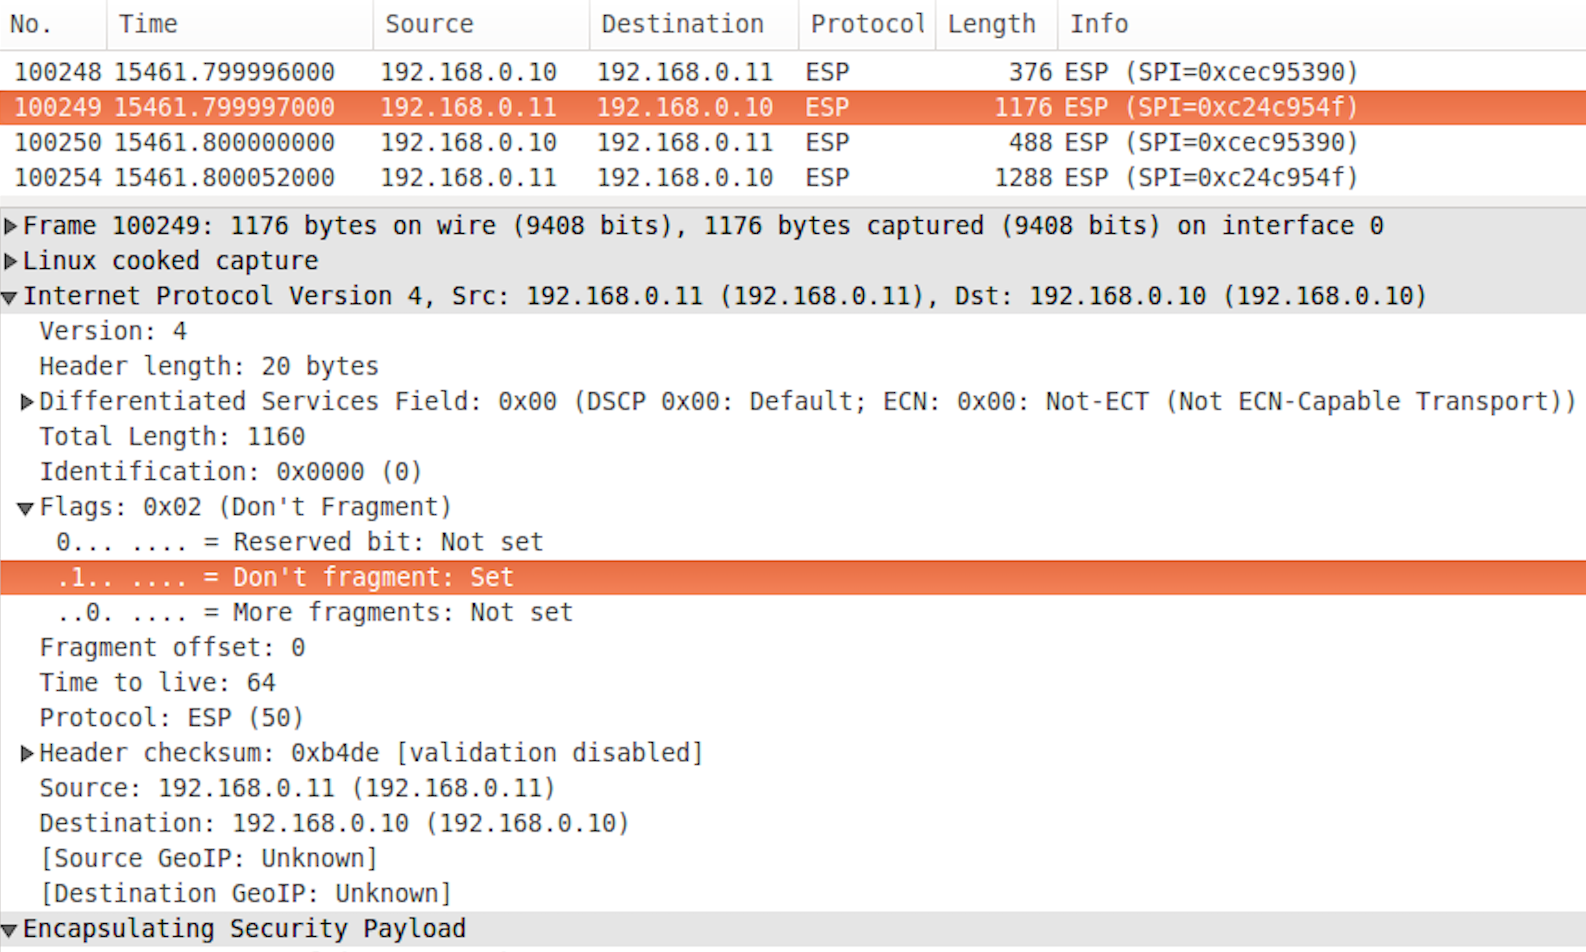
\includegraphics[trim=1 0 0 0,clip,width=\textwidth]{mainpart/implementation/img/ESP_DontFragment}
    \end{center}
    \caption{In ESP gekapseltes ICMP Paket mit \enquote{Don't fragment} flag.}
\end{figure}

Um den \acs{MTU} Discovery Vorgang zu starten wird jeweils ein \enquote{ICMPv4TypeEchoRequest} versendet. Erhält der Ziel Computer das Paket sendet er ein Ping Reply mit dem gleichen Paketinhalt zurück.

\begin{figure}[H]
    \begin{center}
    		% GFX Trim left bottom right top
        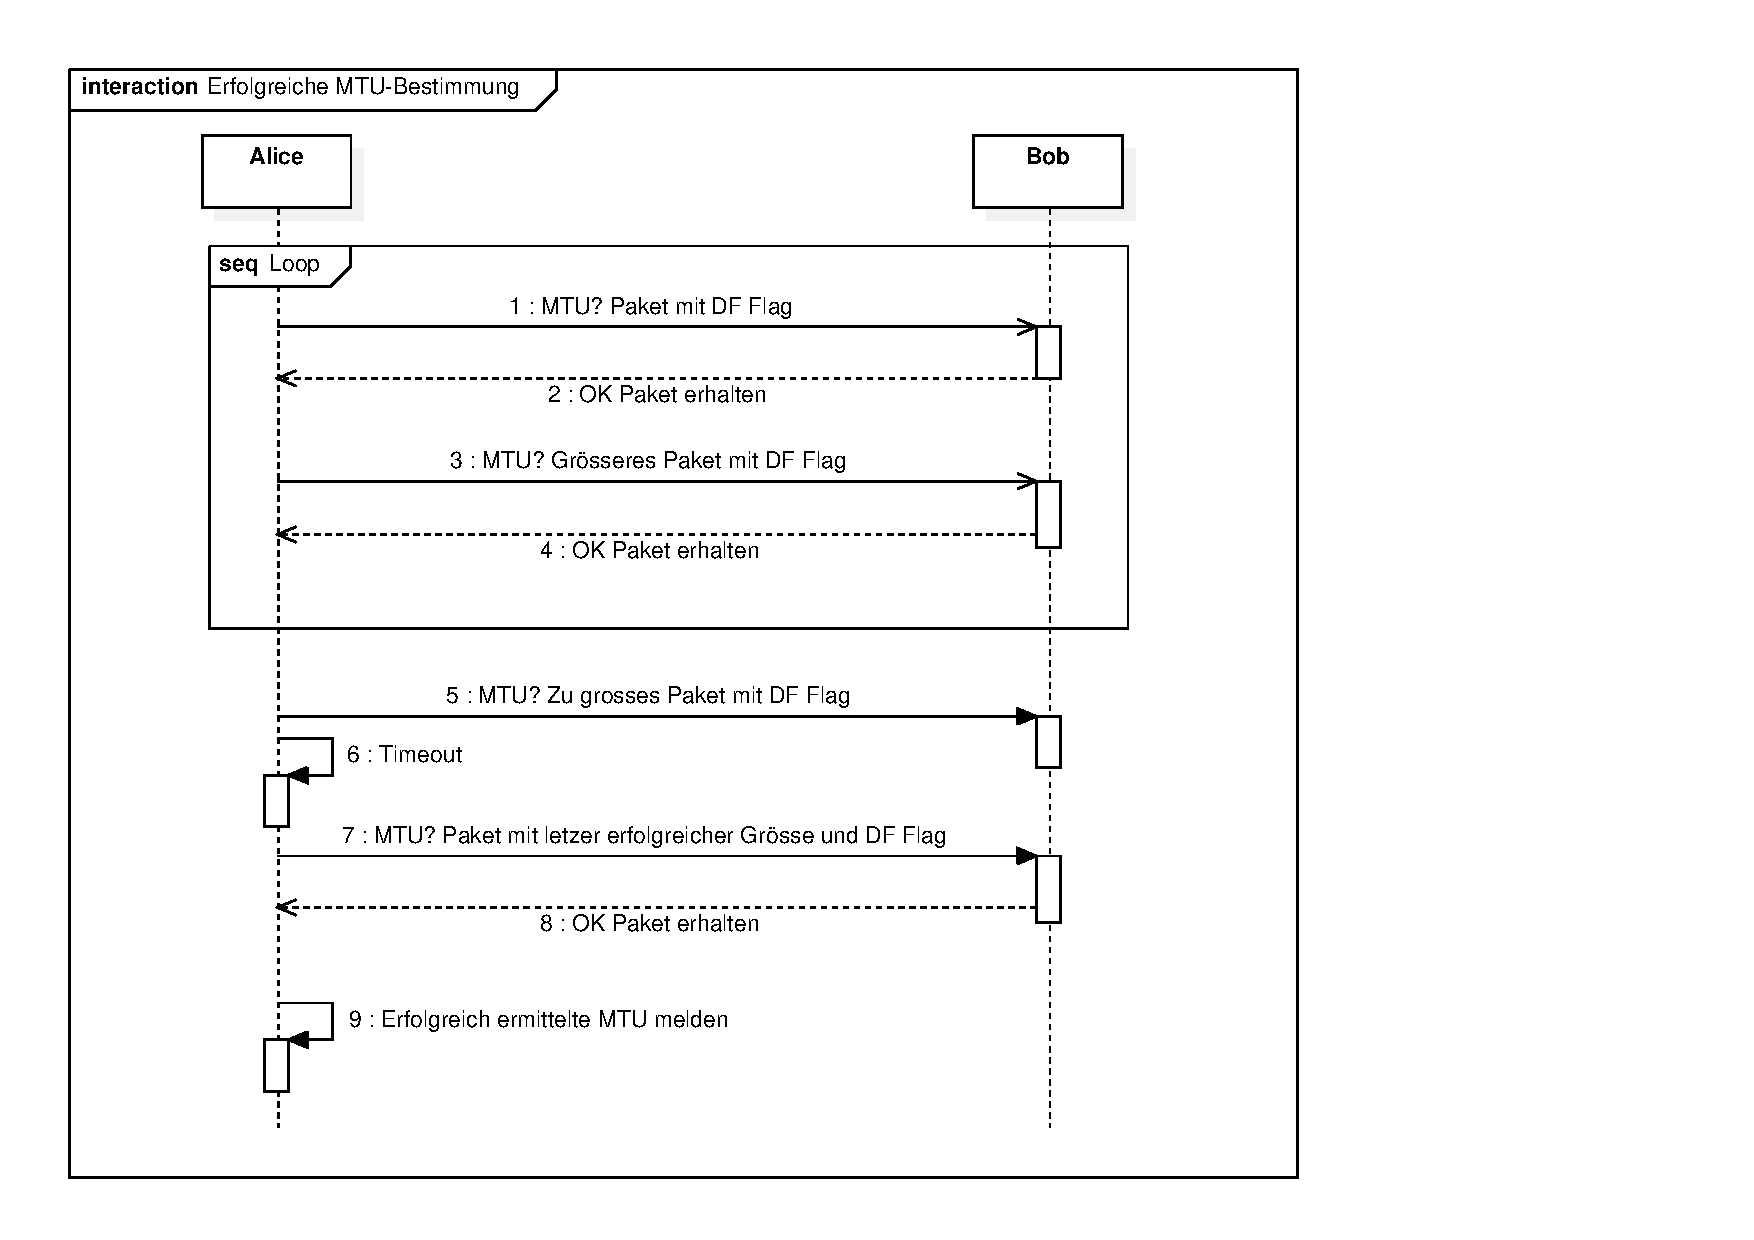
\includegraphics[trim=30 80 140 20,clip,width=\textwidth]{mainpart/implementation/img/MTUBestimmungErfolgreich}
    \end{center}
    \caption{Vereinfachter Ablauf der MTU Bestimmung}
\end{figure}

Die obenstehende Grafik zeigt den weiteren Ablauf der \acs{MTU} Bestimmung mit dem \tool{}. Alice sendet ein \enquote{ICMPv4TypeEchoRequest} Paket einer bestimmten Grösse an Bob. Wenn Bob das Paket erhält, sendet er ein \enquote{ICMPv4TypeEchoReply} Paket mit derselben Grösse als Antwort. Alice erhöht darauf die Paketgrösse und schickt erneut ein \enquote{ICMPv4TypeEchoRequest} an Bob. Dies wird so lange wiederholt bis das Paket nicht mehr ankommt. Bob erhält also das \enquote{ICMPv4TypeEchoRequest} Paket nicht und kann somit Alice auch keine Antwort schicken. Alice wartet nun einen konfigurierten Timeout ab. Wenn innerhalb des Timeouts keine Antwort ankommt geht Alice davon aus, dass das Paket aufgrund der \ac{MTU} von Bob verloren gegangen ist. So lässt sich die \ac{MTU} zwischen Alice und Bob ermitteln.

\subsection{Erster Prototyp mit Binary Search}
Für den ersten Prototyp des \tool{} haben wir die \ac{MTU} Discovery auch wie oben beschrieben implementiert. Es wurden also immer ein Request abgeschickt und dann auf eine Antwort gewartet. Die Idee dabei war die \ac{MTU} mithilfe des Binary Search Algorithmus zu finden. 

\begin{lstlisting}[language=bash, caption=MTU Discovery in Binary Search]                    
Range 0		-	2000 --> Trying 1000
Range 1000	-	2000 --> Trying 1500
Range 1500	-	2000 --> Trying 1750
Range 1500	-	1750 --> Trying 1625
Range 1500	-	1625 --> Trying 1562
Range 1500 	-	1563 --> Trying 1532
Range 1500	-	1532 --> Trying 1516
Range 1500	-	1508 --> Trying 1504
Range 1500	- 	1504 --> Trying 1502
Range 1500	-	1502 --> Trying 1501
Range 1500 	- 	1501 --> Exact MTU detected
\end{lstlisting}

Wie man der Darstellung (oben) entnehmen kann braucht man 11 Versuche um die exakte \ac{MTU} in einem Range von 0-2000 Bytes zu finden. Solange die Antwortszeit zwischen Alice und Bob klein ist, funktioniert diese Art der \ac{MTU} Bestimmung gut und zuverlässig.

Beim Mitte-Projekt Meeting mit dem Industriepartner kam die Frage auf, welches Szenario eintritt, wenn man die \ac{MTU} auf einer sehr langsamen Verbindung feststellen möchte. So betreibt die \osag{} einige Verbindungen, die noch via Satelliten-Link angebunden sind. Bei solchen Verbindungen sind gemäss der \osag{} Timeouts von 10 Sekunden realistisch. Wenn jetzt beim Binary Search Algorithmus für jedes Paket das nicht ankommt auf ein 10 Sekunden Timeout gewartet werden muss, dann dauert die \ac{MTU} Discovery ganz schön lange. Und so haben wir uns nochmals Gedanken gemacht, wie die \ac{MTU} mit einem ähnlichen Algorithmus in wenigen Schritten gefunden werden kann.

\subsection{FastMTU Algorithmus}
Die Lösung des Problems war vergleichsweise einfach. Anstatt wie bei Binary Search den Range nur zu halbieren könnte man ihn in eine konfigurierbare Anzahle Stücke aufteilen. Das Versenden von mehreren Paketen kostet weder Zeit noch nennenswerte Performance. Man kann damit aber einige Versuche sparen und die totale Wartezeit verkürzen. Diesen neuen Algorithmus haben wir "FastMTU" getauft. Bei der nachfolgenden Darstellung ist die Verbesserung durch FastMTU im Vergleich zu BinarySearch ersichtlich.

\begin{lstlisting}[language=bash, caption=FastMTU Discovery]                    
Range 0		-	2000 --> Trying 100, 200, 300, .. 2000
Range 1500	-	1600 --> Trying 1500, 1505, 1510, .. 1600
Range 1500	-	1505 --> Trying 1500, 1501, 1502, .. 1505
\end{lstlisting}

Es werden also nur noch 3 Versuche zum Aufspüren der exakten \ac{MTU} gebraucht werden. Bei einem konfigurierten Timeout von 10 Sekunden würde die \ac{MTU} Discovery im Range 0-2000 immer 30 Sekunden in Anspruch nehmen.

\subsection{Konfigurierte Werte}
Um FastMTU durchführen zu können müssen vom Nutzer folgende Werte konfiguriert werden:

\begin{itemize}
  \item \textbf{Range:} Die \ac{MTU} sollte sich innerhalb des Range befinden.
  \item \textbf{ConcurrentPackets:} Die Anzahl von gleichzeitig verschickten Paketen. Mehr Pakete reduzieren die Anzahl der benötigten Versuche zur Auffindung der \ac{MTU}.
  \item \textbf{Timeout:} Die Zeitdauer die gewartet werden soll zwischen den Versuchen.
\end{itemize}

Ausserdem werden natürlich noch die Source- und Destination-IP Adressen benötigt.

